\documentclass{article}

\usepackage{url} 
\usepackage[normalem]{ulem}

\usepackage{pdfpages}
\usepackage{lastpage}
\usepackage{fancyhdr}
\usepackage{ngerman}

\usepackage{xcolor}
\usepackage{listings}
\usepackage{courier}

\usepackage{floatrow}
\usepackage[tableposition=top]{caption}
\floatsetup[table]{capposition=top}

\usepackage{amsmath, amssymb}

\usepackage[utf8]{inputenc}


\usepackage[numbib]{tocbibind}


\title{Trägheitsmomente}
\author{Johannes Winkler}
\date{}


\newcommand\twodigits[1]{%
   \ifnum#1<10 0#1\else #1\fi
}



\lhead{Trägheitsmomente}
\rhead{\today\\Johannes Winkler}
\cfoot{\twodigits{\thepage}~/ \pageref{LastPage}}

\begin{document}

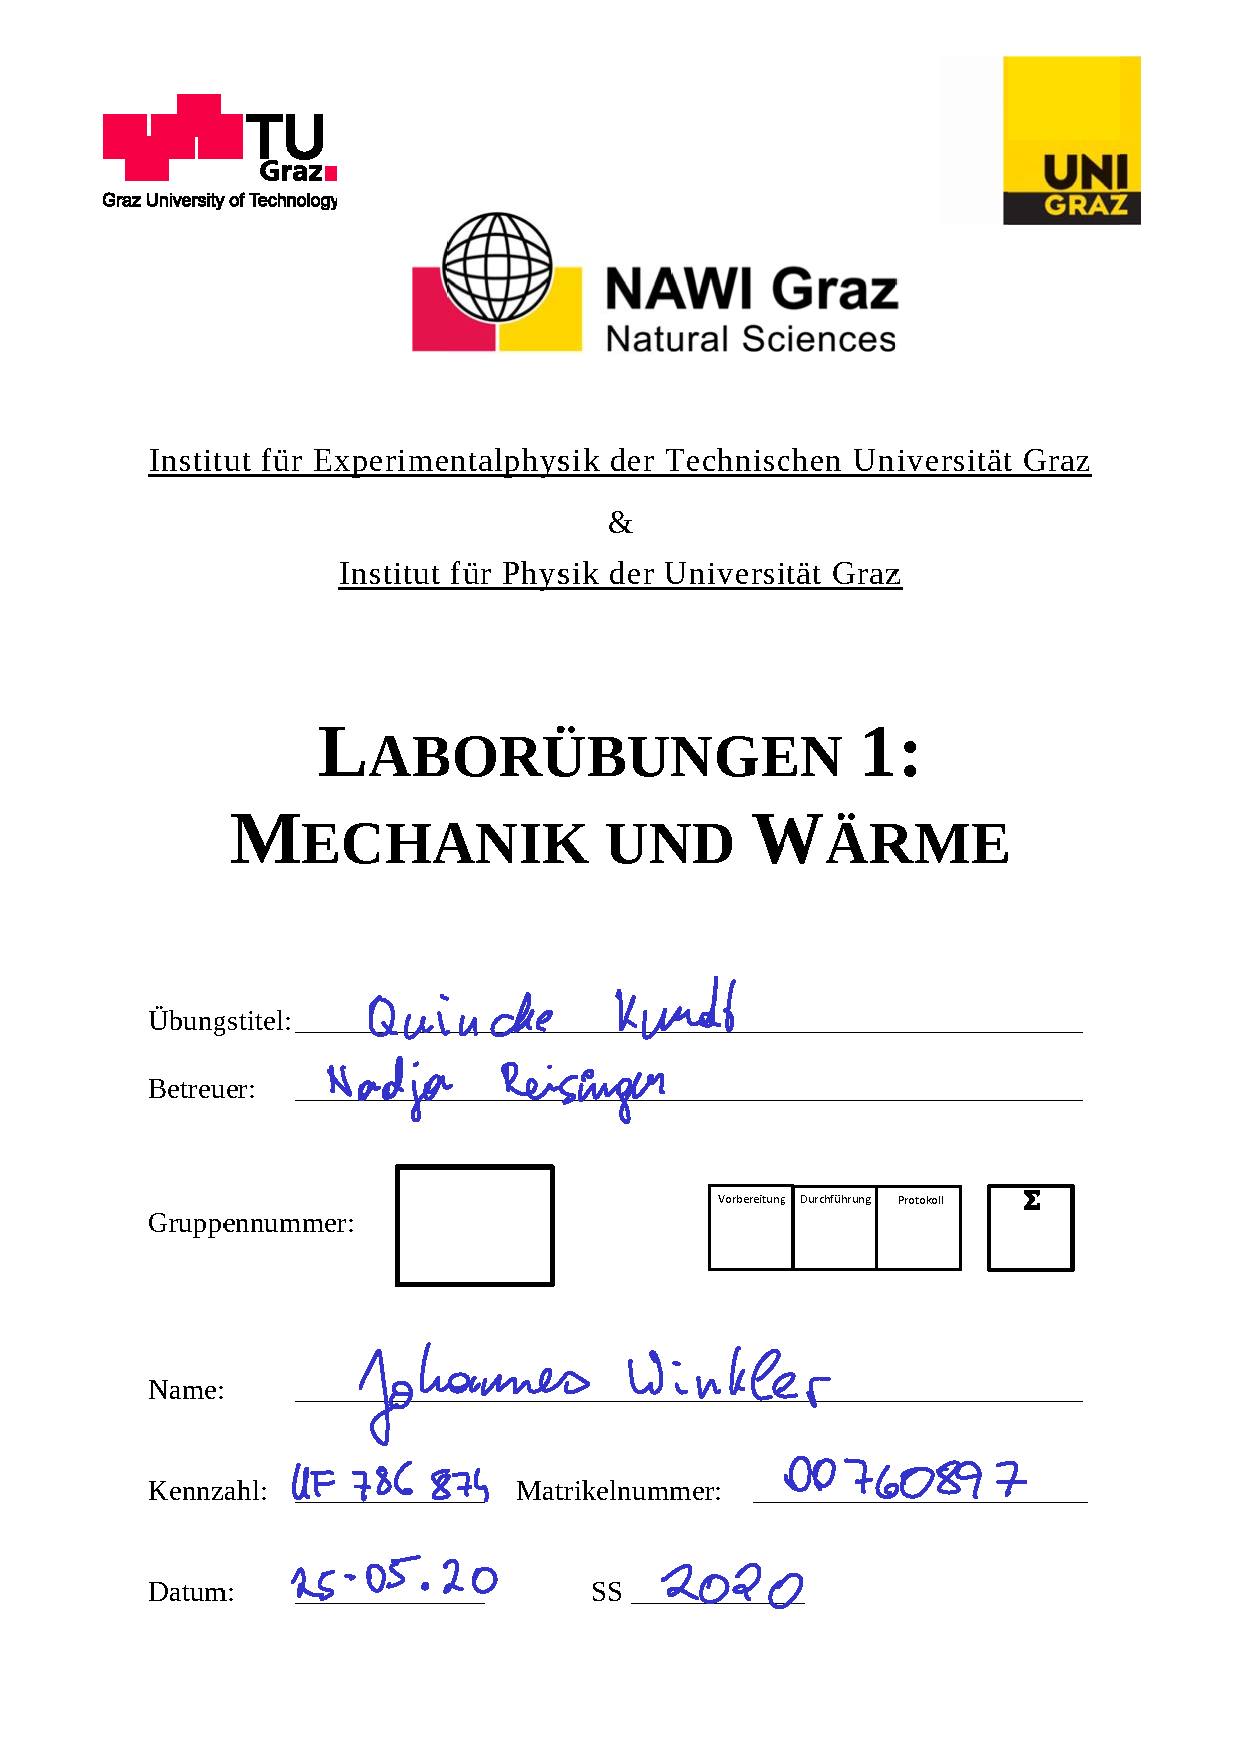
\includepdf[page=-]{deckblatt.pdf} 
 
 
\pagestyle{fancy}


\tableofcontents

\newpage




\section{Aufgabenstellung}
Bestimmen sie für eine Drehschwingung Direktionsmoment $D_r$, Trägheitsmoment $I$, Dämpfung $\gamma$ und Kennfrequenz $\omega_0$. Das schwingende Objekt ist ein iPhone XS Max. 

Als Zuhilfenahme für die Bestimmung des Trägheitsmomentes $I$ werden an das iPhone Batterien angeklebt, dessen Trägheitsmoment $I^\prime$ aufgrund deren geometrischen Beschaffenheit näherungsweise genauer bestimmt werden kann als derer des iPhones.


\section{Grundlagen}
Ein Körper führt eine Drehschwingung um die Achse aus, diese benötigt einige Größen, um sie genau beschreiben zu können. Zum einen gibt es den zurückgelegten Winkel $\varphi$, dieser gibt die momentane Auslenkung an. Bei der Translation gilt, dass Kraft gleich Masse mal Beschleunigung ist, analog gilt für Rotationen
\begin{align}
T = I \cdot \ddot{\varphi}
\end{align}
wobei $T$ das Drehmoment und $I$ das Trägheitsmoment ist.
Das Trägheitsmoment im Allgemeinen ist definiert als
\begin{align}
I = \sum m_i \cdot r_i \qquad \text{oder} \qquad I = \rho \cdot \int r_{\perp}^2 \cdot dV
\end{align}
In unserem Fall werden ein Smartphone (näherungsweise ein Quader) und Batterien (näherungsweise Zylinder) verwendet. Für diese gilt
\begin{align}
I_{\text{Quad}} &= \frac{1}{12}\cdot m \cdot (a^2 + b^2) \\
I_{\text{Zy}} &= \frac{1}{2} \cdot m \cdot r^2
\end{align}
wobei $a,b$ die Abmessungen des Quaders (ausgenommen die Länge in Richtung der Drehachse) und $r$ der Radius des Zylinders ist. Da die Batterien an Rand des Smartphones dazugeklebt werden, müssen diese gemäß Satz von Steiner um die Strecke der halben Smartphonelänge $b/2$ plus den Radius der Batterie $r$ verschoben werden. Dann gilt für das Trägheitsmoment einer nach außen verschobenen Batterie
\begin{align}
I^\prime &= \frac{1}{2}\cdot m\cdot r^2 + m \cdot \left(\frac{b}{2} + r\right)^2 \\
&= \frac{1}{2}\cdot m \cdot r^2 + m\cdot\left(\frac{b^2}{4} + b\cdot r + r^2\right)  \\
&= \frac{1}{4}\cdot m\cdot \left( 2\cdot r^2 + b^2 + 4\cdot b \cdot r + 4\cdot r^2\right) \\
&= \frac{1}{4} \cdot m \cdot \left( 6\cdot r^2 + 4\cdot b \cdot r + b^2\right)
\end{align}
Beim Versuchsaufbau wird darauf geachtet, dass alle Batterien denselben Abstand von der Drehachse haben. Würde man das nicht so machen, dann würde der spätere Ansatz mit der Regression nicht so einfach funktionieren.


~

Die Drehschwingung (ohne Berücksichtigung der Dämpfung) ist gegeben als
\begin{align}
\varphi(t) = \varphi_0 \cdot \cos(\omega_0 \cdot t)
\end{align}
wobei die Frequenz 
\begin{align}
\label{eq:kennfreq}
\omega_0 = \sqrt{\frac{D_r}{I}}
\end{align}
ist. Wegen $\omega_0 = 2\cdot \pi / t$ folgt für die Periodendauer
\begin{align*}
t = 2\cdot \pi \cdot \sqrt{\frac{I}{D_r}}
\end{align*}
Ändert man nun das Trägheitsmoment des Smartphones durch Hinzufügen von $n$ Batterien von $I$ zu $I + n\cdot I^\prime$ ($I^\prime$ ist das Trägheitsmoment einer Batterie), dann ändert sich auch die Periodendauer. Es folgt bei Betrachtung von $t$ in Abhängigkeit von der Anzahl der hinzugefügten Batterien $n$.
\begin{align*}
t(n) &= 2\cdot \pi \cdot \sqrt{\frac{I + n\cdot I^\prime}{D_r}} \\
t^2(n) &= 4\cdot \pi^2 \cdot \frac{I + n\cdot I^\prime}{D_r} \\
t^2(n) &= \underbrace{\frac{4\cdot \pi^2 \cdot I}{D_r}}_{=d} + n\cdot \underbrace{\frac{4\cdot\pi^2 \cdot I^\prime}{D_r}}_{=k}
\end{align*}
Das kann man durch Regression wiederum als Gerade modellieren, sodass $t^2 = d + k\cdot n$ gilt. Das Direktionsmoment erhält man dann aus
\begin{align}
D_r = \frac{4\cdot\pi^2\cdot I^\prime}{k}
\end{align}
Division von $k$ und $d$ liefert
\begin{align}
\frac{d}{k} = \frac{I}{I^\prime}
\end{align}
Wie bereits gesagt, sei $I^\prime$ aufgrund der Geometrie von Batterien leicht(er) zu bestimmen und daher kann für das Trägheitsmoment des iPhones ein Wert abgeleitet werden.

Es wird noch die Dämpfung benötigt. Aus der elementaren Gleichung $A_t = A_0\cdot e^{-\gamma\cdot t}$ folgt
\begin{align}
\gamma = \frac{\ln(A_0) - \ln(A_t)}{t}
\end{align}


Zusätzlich benötigt man noch die Formel für die lineare Regression (inkl. Fehlerabschätzung)



\definecolor{commentgreen}{RGB}{2,112,10}
\definecolor{eminence}{RGB}{108,48,130}
\definecolor{weborange}{RGB}{255,165,0}
\definecolor{frenchplum}{RGB}{129,20,83}

\lstdefinelanguage{elixir}{
    morekeywords={def, for, range, abs, return},
    otherkeywords={<-,->, |>, \%\{, \}, \{, \, (, )},
    sensitive=true,
    morecomment=[l]{\#},
    morecomment=[n]{/*}{*/},
    morecomment=[s][\color{purple}]{:}{\ },
    morestring=[s][\color{orange}]"",
    commentstyle=\color{commentgreen},
    keywordstyle=\color{eminence},
    stringstyle=\color{red},
	basicstyle=\ttfamily,
	breaklines,
	showstringspaces=false,
	frame=tb
}

\begin{lstlisting}[language=elixir, caption={Formel zur Berechnung der Regression.},captionpos=b, label=lst:test]
def regression(x,y):
    xd = sum(x)/len(x)
    yd = sum(y)/len(y)
    zaehler = 0
    nenner = 0
    for i in range(len(x)):
        zaehler += (x[i] - xd) * (y[i] - yd)
        nenner += (x[i] - xd)**2
    k = zaehler / (1.0 * nenner)
    d = yd - k * xd
    return d, k

def regression_fehler(x,y):
    d = [0,0,0]
    k = [0,0,0]
    d[0],k[0] = regression([x[0],x[1]],[y[0],y[1]])
    d[1],k[1] = regression([x[0],x[2]],[y[0],y[2]])
    d[2],k[2] = regression([x[1],x[2]],[y[1],y[2]])
    return spannweite(d)/2, spannweite(k)/2 #delta_d, delta_k

def spannweite(data):
    return max(data) - min(data)
\end{lstlisting}




\paragraph{Kurzusammenfassung der Theorie:}

Bei Durchführung erhält man eine Periodendauer $t(0)$, $t(2)$ und $t(4)$ (abhängig von Anzahl der angeklebten Batterien). Daraus ermittelt man Regressionsgerade $t^2(n) = d + k\cdot n$. Zusätzlich lassen sich die Amplituden messen (=maximale Eindrehung).

Zusätzlich berechnet man das Trägheitsmoment einer Batterie $I^\prime$ aufgrund geometrischer Überlegungen und der Annahme, dass die Dichte homogen ist mit
\begin{align}
I^\prime &= \frac{1}{4} \cdot m \cdot \left( 6\cdot r^2 + 4\cdot b \cdot r + b^2\right).
\end{align}

Aus $I^\prime$, $k$ und $d$ erhält man
\begin{align}
D_r &= \frac{4\cdot\pi\cdot I^\prime}{k} \\
I &= \frac{d}{k}\cdot I^\prime
\end{align}
und aus der Amplitude erhält man
\begin{align}
\gamma &= \frac{\ln(A_0) - \ln(A_t)}{t}
\end{align}
Schließlich erhält man auch noch 
\begin{align}
\omega_0 = \sqrt{\frac{D_r}{I}}
\end{align}


\section{Beschreibung der Versuchsanordnung}

Für die Abmessungen der benutzten Batterien wird darauf vertraut, dass sich der Hersteller Duracell an die offiziellen Spezifikationen (\cite{duracell}) hält. Trotzdem wird im Sinne der Fehlerrechnung ein Messfehler von $0.1~$mm angenommen. Diesselben Annahmen werden beim Apple iPhone XS Max getroffen (vgl. \cite{apple}).




\section{Geräteliste}




\begin{table}[H]
\caption{Geräteliste}



\begin{tabular}{lll}
Gerät  & Beschreibung \\
\hline
Küchenwaage & von Firma Soehnle, digitales Display, max. Gewicht 5~kg \\
iPhone XS max & Apple, (77.4~mm x 157.5~mm x 7.7~mm, Masse: 208~g)\\
Faden & Farbe: weiß, Material: Nylon \\
4 AAA Batterien & Hersteller Duracell, h: 44.5 mm, r: 5.25 mm, Masse: 11~g \\
Lineal & Geodreieck Aristo \\
Schiebelehre & kein Hersteller erkennbar
\end{tabular}
\end{table}

\newpage
\section{Versuchsdurchführung und Messergebnisse}

Das iPhone wird 10 mal um die eigene Achse gedreht und dann los gelassen. Es wurde über mehrere Perioden die Zeit gestoppt und dann die Dauer einer Periode gemittelt. Die Ergebnisse sind in Tabelle \ref{tab:periodendauer} aufgelistet.


\begin{table}[H]
\caption{Messung der Periodendauer}
\label{tab:periodendauer}
\begin{tabular}{l|l}
& Periodendauer / s \\
\hline
ohne Batterien & 17.6 \\
2 Batterien & 27.8 \\
4 Batterien & 32.5
\end{tabular}
\end{table}

Die Amplitude ist in dem gegebenen Kontext ein Maß für die \textit{maximale Einwicklung}. D.h. Zu Beginn des Versuchs ist die Amplitude $A_0 = 2\cdot \pi \cdot 10$, also 10 volle Umdrehungen. Nach $17.7$ Sekunden war das zweite Maximum bei nur noch $8.4$ Umdrehungen, also $A_{17.7} = 2\cdot \pi \cdot 8.4$.





\newpage
\section{Auswertung}

Zuerst muss die das Trägheitsmoment von Batterien bestimmt werden. Dieses ist aufgrund der Verschiebung
\begin{align}
I^\prime &= \frac{1}{4} \cdot m \cdot \left( 6\cdot r^2 + 4\cdot b \cdot r + b^2\right) = 77.77~\text{mg m}^2
\end{align}
Die nötigen Größen wurden aus der jeweiligen Spezifikation (\cite{apple}, \cite{duracell}), wurden aber mit einer Küchenwaage und einer Schiebelehre nachgemessen und stimmen mit den Werten aus der Spezifikation überein. Trotzdem lässt sich eine Unsicherheitsanalyse machen, wenn man z.B. für die Längenmessung $\Delta \ell = 0.1~$mm und für die Massenbestimmung $\Delta m = 0.1$~g ansetzt. Durch die Größtunsicherheitsmethode erhält man
\begin{align}
\Delta I^\prime = \frac{1}{4}\cdot \bigg[\Delta m \cdot \left( 6\cdot r^2 + 4\cdot b \cdot r + b^2\right) + m \cdot \left( 12\cdot r + 4\cdot b \right)\cdot \Delta r \\ 
+ m \cdot \left(  4 \cdot r + 2\cdot b\right)\cdot \Delta b\bigg] = 0.99~\text{mg m}^2
\end{align}

Danach kann die Regression bestimmt werden. Die berechneten Parameter sind
\begin{align}
k &= 186.62~\text{s}^2 \\
d &= 339.71~\text{s}^2
\end{align}
Die Regressionsgerade kann auch gezeichnet werden.

\begin{figure}[H]
\centering
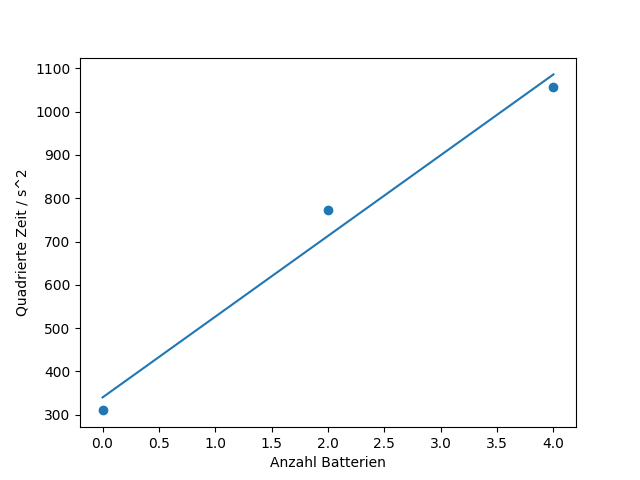
\includegraphics[height=7cm]{regression.png}
\caption{Regressionsgerade}
\end{figure}

Für die Unsicherheit von $k$ und $d$ wird die Regression auf verschiedene Arten mit 2 der 3 Punkten berechnet. Die Abweichungen der Werte für $k$ und $d$ werden dann als Unsicherheit verwendet. Insgesamt gilt
\begin{align}
\Delta k &= 44.92~\text{s}^2\\
\Delta d &= 89.84~\text{s}^2
\end{align}




Für das Direktionsmoment gilt
\begin{align}
D_r &= \frac{4\cdot\pi\cdot I^\prime}{k} &= 5.24~\mu\text{Nm}\\
\Delta D_r &= 4\cdot\pi\cdot \left[ \frac{\Delta I^\prime}{k} + \frac{I^\prime}{k^2}\cdot \Delta k \right]  &= 1.33~\mu\text{Nm}
\end{align}
Ebenfalls durch Größtunsicherheitsmethode gilt
\begin{align}
I &= \frac{d}{k}\cdot I^\prime  &= 141.56~\text{mg m}^2 \\
\Delta I &= \frac{\Delta d}{k}\cdot I^\prime +\frac{d}{k^2}\cdot I^\prime\cdot \Delta k +\frac{d}{k}\cdot \Delta I^\prime &= 73.31~\text{mg m}^2 
\end{align}
Für die Dämpfung gilt 
\begin{align}
\gamma &= \frac{\ln(A_0) - \ln(A_t)}{t} = \frac{\ln(A_0 / A_{17.7})}{17.7} = 9.85\cdot 10^{-3}~\text{s}^{-1}
\end{align}
Die Unsicherheit der Dämpfung ist
\begin{align}
\Delta \gamma &= \left| \frac{\partial \gamma}{\partial A_0} \right|\cdot \Delta A_0 + \left| \frac{\partial \gamma}{\partial A_1} \right|\cdot \Delta A_1 + \left| \frac{\partial \gamma}{\partial t} \right|\cdot \Delta A_t \\
&= \frac{\Delta A_0}{A_0 \cdot t} +\frac{\Delta A_1}{A_1 \cdot t} + \frac{\ln(A_0) - \ln(A_1)}{t^2}\cdot \Delta t = 0.17\cdot10^{-3}~\text{s}^{-1}
\end{align}
Für den Fehler der Zeitmessung wird 1 Millisekunde angenommen, für die Winkelmessung $5~^\circ$.
Es ergibt sich die Kennfrequenz aus Formel \eqref{eq:kennfreq}
\begin{align}
\omega_0 &= \sqrt{\frac{D_r}{I}}  = 0.19~\text{s}^{-1} \\
\Delta \omega_0 &= \frac{1}{2} \cdot \sqrt{\frac{I}{D_r}} \cdot \frac{\Delta D_r}{I} + \frac{1}{2}\cdot  \sqrt{\frac{I}{D_r}} \cdot \frac{D_r}{I^2}\cdot \Delta I  \\
&= \frac{0.5}{\omega_0 \cdot I} \cdot \left( \Delta D_r + \frac{D_r}{I}\cdot \Delta I \right) = 0.07~\text{s}^{-1}
\end{align}


Abschließend kann das Trägheitsmoment des iPhones unter Annahme einer homogenen Dichte und der Form eines Quaders auch direkt berechnet werden. Runde Ecken werden ebenfalls vernachlässigt.
\begin{align*}
I^* &= \frac{1}{12}\cdot m \cdot (a^2 + b^2) = 431~\text{mg m}^2 \\
\Delta I^* &= \frac{1}{12}\cdot \left( \Delta m \cdot (a^2 + b^2) + 2\cdot m \cdot (a\cdot \Delta a + b \cdot \Delta b)  \right) = 0.78~\text{mg m}^2
\end{align*}



\newpage
\section{Zusammenfassung und Diskussion}

Für die Auswertung einer nach außen verschobenen Batterie ergibt sich
\begin{align*}
I^\prime = (77.77 \pm 0.99)~\text{mg m}^2
\end{align*}
Hierfür verwendet man Masse und Abmessungen aus der Spezifikation \cite{duracell}. Durch die exakten Angaben in der Spezifikation ist die Unsicherheit sehr klein im Vergleich zum Ergebnis. Für Direktionsmoment und Dämpfung gilt
\begin{align}
D_r &= (5.24 \pm 1.33)~\mu\text{Nm} \\
\gamma &= (9.85 \pm 0.17)\cdot 10^{-3} ~\text{s}^{-1}
\end{align}
Die Kennfrequenz beträgt
\begin{align}
\omega_0 &= (0.19 + 0.07)~\text{s}^{-1}
\end{align}
Für das Trägheitsmoment des iPhones erhält man
\begin{align}
I &= (141.56 \pm 72.31)~\text{mg~m}^2 \\
I^* &= (431 \pm 0.78)~\text{mg~m}^2
\end{align}
Man sieht hier, dass der gemessene Wert $I$ trotz der hohen Unsicherheit nicht an den theoretischen Wert heran kommt. Das liegt daran, dass für den theoretischen Wert die Geomtrie und der Aufbau des Gerätes nicht berücksichtigt wurden.

Die hohe Unsicherheit an $I$ liegt unter anderem auch daran, dass für die Regression ein sehr großer Fehler angenommen wurde. Durch mehrere Gewichter könnte man ein genaueres Ergebnis liefern.

\begin{thebibliography}{9}
\bibitem{demtr1} W. Demtröder, \emph{Experimentalphysik 1: Mechanik und Wärme}, Springer-Spektrum, 8. Auflage, 2018.

\bibitem{giancoli} D. Giancoli, \emph{Physik}, Pearson, 4. Auflage, 2019.

\bibitem{apple} \url{https://support.apple.com/kb/SP780?locale=de_AT} (Stand: \today)

\bibitem{duracell} \url{https://www.batterijenhuis.nl/image/data/datasheets/duracell/Datasheet-Duracell-Plus-Power-AAA.pdf} (Stand: \today) 

\end{thebibliography}

\end{document}
